% Drishti conference paper. Built on the official IEEEtran conference template
% (IEEEtran.cls v1.8b, IEEEtran.bst v1.14, CTAN 2015/08/26); bare_conf.tex in template/.
% Build: python3 scripts/numbers.py && pdflatex main && bibtex main && pdflatex main && pdflatex main
\documentclass[conference]{IEEEtran}
\IEEEoverridecommandlockouts

\usepackage[T1]{fontenc}
\usepackage{cite}
\usepackage{amsmath,amssymb,amsfonts}
\usepackage{graphicx}
\usepackage{textcomp}
\usepackage{xcolor}
\usepackage{booktabs}
\usepackage{tikz}
\usetikzlibrary{positioning,fit,arrows.meta,calc}
\usepackage{pgfplots}
\pgfplotsset{compat=1.17}
\graphicspath{{figures/}}

% Drafting marker; removed before submission.
\newcommand{\todo}[1]{\textcolor{red}{[TODO: #1]}}
% Generated by scripts/numbers.py from data/. Do not edit.
\newcommand{\synDepN}{90}
\newcommand{\synDepCorrect}{84}
\newcommand{\synDepCorrectPct}{93}
\newcommand{\synDepCorrectCI}{86--97}
\newcommand{\synDepWrong}{6}
\newcommand{\synDepRejected}{0}
\newcommand{\synDepDeclined}{0}
\newcommand{\synDepRtMed}{0.9}
\newcommand{\synDepRtNinetyFive}{2.3}
\newcommand{\synDepRtMax}{4.4}
\newcommand{\synDepTokens}{894}
\newcommand{\synDepBytes}{4.6}
\newcommand{\synDepKeysOk}{all}
\newcommand{\synDepTrialsSame}{identical}
\newcommand{\synDepTrialCorrect}{28}
\newcommand{\synDepTrialN}{30}
\newcommand{\synDepTrialCI}{79--98}
\newcommand{\synFreeN}{90}
\newcommand{\synFreeCorrect}{79}
\newcommand{\synFreeCorrectPct}{88}
\newcommand{\synFreeCorrectCI}{79--93}
\newcommand{\synFreeWrong}{8}
\newcommand{\synFreeRejected}{3}
\newcommand{\synFreeDeclined}{0}
\newcommand{\synFreeRtMed}{0.9}
\newcommand{\synFreeRtNinetyFive}{3.5}
\newcommand{\synFreeRtMax}{6.6}
\newcommand{\synFreeTokens}{869}
\newcommand{\synFreeBytes}{3.2}
\newcommand{\synFreeKeysOk}{all}
\newcommand{\synFreeTrialsSame}{different}
\newcommand{\synFreeTrialCorrect}{26}
\newcommand{\synFreeTrialN}{30}
\newcommand{\synFreeTrialCI}{70--95}
\newcommand{\synThinkN}{90}
\newcommand{\synThinkCorrect}{65}
\newcommand{\synThinkCorrectPct}{72}
\newcommand{\synThinkCorrectCI}{62--80}
\newcommand{\synThinkWrong}{3}
\newcommand{\synThinkRejected}{11}
\newcommand{\synThinkDeclined}{11}
\newcommand{\synThinkRtMed}{5.5}
\newcommand{\synThinkRtNinetyFive}{29.2}
\newcommand{\synThinkRtMax}{36.8}
\newcommand{\synThinkTokens}{2,276}
\newcommand{\synThinkBytes}{4.4}
\newcommand{\synThinkKeysOk}{all}
\newcommand{\synThinkTrialsSame}{different}
\newcommand{\synThinkTrialCorrect}{22}
\newcommand{\synThinkTrialN}{30}
\newcommand{\synThinkTrialCI}{56--86}
\newcommand{\synUltraN}{90}
\newcommand{\synUltraCorrect}{90}
\newcommand{\synUltraCorrectPct}{100}
\newcommand{\synUltraCorrectCI}{96--100}
\newcommand{\synUltraWrong}{0}
\newcommand{\synUltraRejected}{0}
\newcommand{\synUltraDeclined}{0}
\newcommand{\synUltraRtMed}{2.4}
\newcommand{\synUltraRtNinetyFive}{5.8}
\newcommand{\synUltraRtMax}{38.5}
\newcommand{\synUltraTokens}{893}
\newcommand{\synUltraBytes}{4.6}
\newcommand{\synUltraKeysOk}{all}
\newcommand{\synUltraTrialsSame}{identical}
\newcommand{\synUltraTrialCorrect}{30}
\newcommand{\synUltraTrialN}{30}
\newcommand{\synUltraTrialCI}{89--100}
\newcommand{\oldBudgetN}{31}
\newcommand{\oldBudgetCut}{8}
\newcommand{\evalEightMed}{12}
\newcommand{\evalEightNinetyNine}{19}
\newcommand{\evalThirtyMed}{44}
\newcommand{\evalThirtyNinetyNine}{70}
\newcommand{\evalSixtyFourMed}{91}
\newcommand{\evalSixtyFourNinetyNine}{137}
\newcommand{\evalMaxMs}{2.0}
\newcommand{\relayOnN}{88}
\newcommand{\relayOnMed}{3.90}
\newcommand{\relayOnNinetyNine}{3.95}
\newcommand{\relayOnMax}{4.47}
\newcommand{\relayOnGpio}{0.13}
\newcommand{\relayOnBounce}{0.44}
\newcommand{\relayOffN}{88}
\newcommand{\relayOffMed}{3.59}
\newcommand{\relayOffNinetyNine}{3.62}
\newcommand{\relayOffMax}{3.77}
\newcommand{\relayOffGpio}{0.13}
\newcommand{\relayOffBounce}{0.05}
\newcommand{\relayRequestedOn}{200}
\newcommand{\relayHeld}{112}
\newcommand{\relayEdges}{1380}
\newcommand{\replayTicks}{172,800}
\newcommand{\replaySameHash}{identical}
\newcommand{\replayRefRules}{28}
\newcommand{\replayStatedMatched}{52}
\newcommand{\replayStatedFalse}{1}
\newcommand{\replayStatedMissed}{2}
\newcommand{\replayStatedRules}{21}
\newcommand{\replayStatedIdentical}{19}
\newcommand{\replayVagueMatched}{11}
\newcommand{\replayVagueFalse}{7}
\newcommand{\replayVagueMissed}{4}
\newcommand{\replayLampAgree}{83.6}
\newcommand{\replayFanAgree}{93.9}
\newcommand{\replayHeld}{0}
\newcommand{\offSeconds}{600}
\newcommand{\offChecks}{120}
\newcommand{\offChecksOnline}{0}
\newcommand{\offSwitches}{9}
\newcommand{\offSwitchesMatched}{9}
\newcommand{\offLagMax}{173}
\newcommand{\egAgentReq}{72}
\newcommand{\egAgentCarry}{72}
\newcommand{\egAgentKb}{16.9}
\newcommand{\egCompileReq}{25}
\newcommand{\egCompileCarry}{0}
\newcommand{\egCompileKb}{3.8}
\newcommand{\egTurns}{30}
\newcommand{\egProposals}{25}
\newcommand{\egAuthorMed}{3.0}
\newcommand{\egAuthorNinetyFive}{11.0}
\newcommand{\cfPairs}{127}
\newcommand{\cfReal}{62}
\newcommand{\cfFlagged}{98}
\newcommand{\cfPrecision}{63}
\newcommand{\cfRecall}{100}
\newcommand{\cfPrompts}{25}
\newcommand{\cfPromptsReal}{18}
\newcommand{\mEmbCorrect}{68}
\newcommand{\mEmbWrong}{13}
\newcommand{\mEmbNovel}{81}
\newcommand{\mEmbNovelN}{120}
\newcommand{\mEmbMs}{2.8}
\newcommand{\mFuzCorrect}{25}
\newcommand{\mFuzWrong}{21}
\newcommand{\rtHand}{49}
\newcommand{\rtHandN}{50}
\newcommand{\rtHandSureWrong}{0}
\newcommand{\rtHeld}{636}
\newcommand{\rtHeldN}{717}
\newcommand{\rtHeldSureWrong}{8}
\newcommand{\rtLitHand}{30}
\newcommand{\rtLitHandN}{50}
\newcommand{\rtLitHandSureWrong}{2}
\newcommand{\rtLitHeld}{103}
\newcommand{\rtLitHeldN}{717}
\newcommand{\rtLitHeldSureWrong}{50}
\newcommand{\rtHandMs}{12.8}
\newcommand{\rtHeldMs}{17.7}
\newcommand{\blN}{59}
\newcommand{\blCorrect}{48}
\newcommand{\blEdges}{19}
\newcommand{\blEdgeCorrect}{11}
\newcommand{\blSpurious}{3}
\newcommand{\blMed}{0.4}
\newcommand{\blNinetyFive}{2.5}
\newcommand{\blMax}{15.6}
\newcommand{\blSlow}{9}
\newcommand{\blTokens}{790}
\newcommand{\blTokensDay}{136}
\newcommand{\blEvents}{1,560}
\newcommand{\blEventTokens}{1.2}

\newcommand{\hcell}[1]{\begin{tabular}[b]{@{}c@{}}#1\end{tabular}}

\begin{document}

\title{Compile Once, Act Locally: Keeping a Cloud Language Model off the
Actuation Path of an Edge Home-Automation System}

\author{%
\IEEEauthorblockN{Veera Manikanta}
\IEEEauthorblockA{\textit{School of Electrical Engineering}\\
\textit{Manipal Institute of Technology, Manipal Academy of Higher Education}\\
Manipal, India\\
\todo{email}}
\and
\IEEEauthorblockN{Sumir Subash Balakrishnan}
\IEEEauthorblockA{\textit{School of Electrical Engineering}\\
\textit{Manipal Institute of Technology, Manipal Academy of Higher Education}\\
Manipal, India\\
\todo{email}}
}

\maketitle

\begin{abstract}
Language-model home assistants either keep the model in the decision loop,
paying seconds of delay and a cloud call for every switch, or turn a sentence
into an automation rule and stop measuring once the rule is stored. We present
an edge system in which a cloud model compiles a spoken or typed instruction
into a typed rule once, an on-device gate checks the rule against the house's
own device registry before a person confirms it, and a local evaluator fires it
with no model and no network. On a Raspberry Pi~5 with a camera-derived room
state and a two-channel relay, the deployed compiler produced a correct rule for
\synDepTrialCorrect{} of \synDepTrialN{} requests with a median round trip of
\synDepRtMed{}~s, and no malformed rule reached the store. Holding the model to
a JSON schema and switching its reasoning off mattered more than the choice of
model: with reasoning on, \synThinkRejected{} of 90 compilations were cut off
before the rule was written. From a firing decision to the relay contact took
\relayOnMed{}~ms, of which \relayOnGpio{}~ms was software. With the network
removed for \offSeconds{}~s the house switched \offSwitches{} times, each by its
rule, and a 24-hour replay produced a byte-identical switching log with and
without a network interface. A model asked to make the same decisions live was
right at only \blEdgeCorrect{} of \blEdges{} switching moments.
\end{abstract}

\begin{IEEEkeywords}
edge computing, home automation, large language models, trigger-action
programming, structured output, offline operation
\end{IEEEkeywords}

% ---------------------------------------------------------------------------
\section{Introduction}\label{sec:intro}

A home assistant built on a large language model (LLM) understands requests
that no fixed grammar anticipates: ``turn the fan off once the room has been
empty for five minutes'' needs no template. The obvious way to use such a model
is to ask it what to do whenever something changes. That places a cloud call,
seconds of variable delay and a per-call cost on every switching decision, and
it stops the house when the network does. The alternative, already explored by
several systems~\cite{chatiot,giudici,autoiot,farm}, is to let the model write
a rule that a conventional runtime executes. Those systems are evaluated at the
point of generation: whether the rule parses, whether the platform accepts it,
how many tokens it costs. What happens after the rule is stored, how fast it
acts, whether it still acts without a network, and how many rules pass every
check yet mean something other than what was said, is rarely reported.

We report it for one complete system. A cloud model compiles an instruction
into a typed rule over a small vocabulary of room-state fields. The rule passes
an on-device gate derived from the house's device registry, is shown to a
person for confirmation, and is then evaluated twice a second against a state
vector built from a camera on the same board. No model and no network sit
between a state change and a relay. Immediate commands (``fan off now'') still
go to the model, with a small on-device router as fallback; we treat that lane
as context and measure the rule lane.

\begin{itemize}
\item We describe a two-lane architecture that keeps a cloud LLM off the
firing path of standing rules, with an edge-triggered evaluator and a switch
guard in front of the relays (Section~\ref{sec:design}).
\item We measure the gate end to end: correct, valid-but-wrong and rejected
compilations for four model settings, and the conflict check against
exhaustive ground truth (Sections~\ref{sec:compile} and~\ref{sec:reuse}).
\item We measure the firing path on real hardware: decision-to-contact time on
a relay, a 10-minute physical test with the network removed, a 24-hour replay
with and without a network interface, and the same decisions made by the model
in the loop (Sections~\ref{sec:latency} and~\ref{sec:offline}).
\end{itemize}

% ---------------------------------------------------------------------------
\section{Related Work}\label{sec:related}

\textit{Model in the loop.} Sasha~\cite{sasha} answers vague goals with a
multi-step LLM pipeline; IoTGPT~\cite{iotgpt} decomposes commands into reusable
subtasks over SmartThings and reports lower command-generation latency and cost
than earlier agents. SAGE~\cite{sage} lets the model write condition code that
is polled, then hands control back to the model to plan the action. Local
variants run a small model on the device~\cite{birkmose,harmony,homellama,adahome},
trading model capability for privacy; the model still decides each command.

\textit{One-time synthesis.} ChatIoT~\cite{chatiot} generates trigger-action
programs for a runtime from conversation; Giudici et al.~\cite{giudici} generate
Home Assistant automations and time the LLM call; AutoIoT~\cite{autoiot} adds
formal verification to detect and repair conflicts among generated rules;
FARM~\cite{farm} maps instructions to IFTTT-style applets; LLMind~\cite{llmind}
stores generated control scripts for reuse; AutoIOT~\cite{autoiot_nl} and
GPIoT~\cite{gpiot} synthesise sensing programs that then run locally. Their
evaluations end at generation (Table~\ref{tab:related}).

\textit{Rule safety and reuse.} Conflict and interaction analysis of
trigger-action rules predates LLMs~\cite{iruler,autotap}; LLMs are weaker than
static analysis at threats that span several rules~\cite{quantrill}. Our
conflict check is deliberately simple and we do not claim it as new. Semantic
caches skip a model call when a request resembles an earlier one and report
wrong hits alongside savings~\cite{gptcache,meancache}. Constrained decoding
holds generation to a grammar or JSON schema~\cite{outlines,xgrammar}, and its
effect varies widely across schemas and engines~\cite{jsonschemabench}.

\begin{table}[t]
\caption{Where the model sits and what is measured after generation}
\label{tab:related}
\centering\footnotesize
\setlength{\tabcolsep}{3pt}
\begin{tabular}{@{}lcccc@{}}
\toprule
System & Stored & \hcell{Model\\at firing} & Offline & \hcell{Actuation\\time}\\
\midrule
SAGE~\cite{sage} & condition code & yes & no & no\\
IoTGPT~\cite{iotgpt} & subtasks & yes & no & no\\
On-device~\cite{birkmose,homellama} & no & local & n.r. & n.r.\\
ChatIoT~\cite{chatiot} & TAP program & no & n.r. & n.r.\\
Giudici~\cite{giudici} & automation & no & no & no\\
AutoIoT~\cite{autoiot} & verified rule & no & no & no\\
This work & typed rule & no & 600~s & 3.9~ms\\
\bottomrule
\end{tabular}\\[2pt]
\raggedright\scriptsize n.r.: not reported in the source available to us (full
text for SAGE, IoTGPT, Giudici et al.\ and AutoIoT; abstract otherwise).
\end{table}

% ---------------------------------------------------------------------------
\section{System Design}\label{sec:design}

Figure~\ref{fig:arch} shows the two lanes. Everything below the dashed line
runs on a Raspberry Pi~5 (16~GB) with a Hailo-8L neural accelerator, a Camera
Module~3 and a two-channel relay board; the cloud side is NVIDIA's hosted
\texttt{nemotron-3.5-super-vl-120b} with \texttt{nemotron-3-ultra-550b} as
fallback.

\begin{figure}[t]
\centering
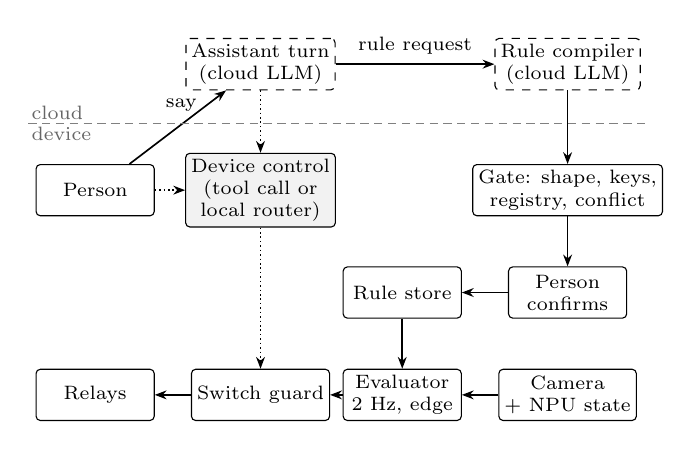
\begin{tikzpicture}[font=\scriptsize,
  box/.style={draw, rounded corners=1.5pt, align=center, inner sep=2pt, minimum height=6.5mm, minimum width=15mm},
  cloud/.style={box, dashed},
  arr/.style={-{Stealth[length=1.5mm]}, semithick},
  imm/.style={arr, densely dotted}]
\node[cloud] (A) at (2.2,0) {Assistant turn\\(cloud LLM)};
\node[cloud] (C) at (6.1,0) {Rule compiler\\(cloud LLM)};
\node[box]   (P) at (0.1,-1.6) {Person};
\node[box, fill=black!5] (R) at (2.2,-1.6) {Device control\\(tool call or\\local router)};
\node[box]   (G) at (6.1,-1.6) {Gate: shape, keys,\\registry, conflict};
\node[box]   (S) at (4.0,-2.9) {Rule store};
\node[box]   (K) at (6.1,-2.9) {Person\\confirms};
\node[box]   (W) at (0.1,-4.2) {Relays};
\node[box]   (U) at (2.2,-4.2) {Switch guard};
\node[box]   (E) at (4.0,-4.2) {Evaluator\\2 Hz, edge};
\node[box]   (M) at (6.1,-4.2) {Camera\\+ NPU state};
\draw[arr] (P) -- node[left, pos=0.8]{say} (A);
\draw[arr] (A) -- node[above]{rule request} (C);
\draw[arr] (C) -- (G);
\draw[arr] (G) -- (K);
\draw[arr] (K) -- (S);
\draw[arr] (S) -- (E);
\draw[arr] (M) -- (E);
\draw[arr] (E) -- (U);
\draw[arr] (U) -- (W);
\draw[imm] (A) -- (R);
\draw[imm] (P) -- (R);
\draw[imm] (R) -- (U);
\draw[densely dashed, black!50] (-0.75,-0.75) -- (7.15,-0.75);
\node[anchor=south west, black!60, inner sep=1pt] at (-0.75,-0.75) {cloud};
\node[anchor=north west, black!60, inner sep=1pt] at (-0.75,-0.75) {device};
\end{tikzpicture}
\caption{Two lanes. Solid: a standing rule is compiled once in the cloud, gated
and confirmed on the device, then fired locally with no model or network.
Dotted: an immediate command is decided by the model, or by an on-device router
when the model is unreachable.}
\label{fig:arch}
\end{figure}

\subsection{State and rules}
Each half second the device builds a state vector from the camera and the
house: occupancy, person count, dwell time, the zone and posture of the largest
person box, ambient light from the image, hour of day, owner presence, optional
sensor readings and the state of every registered device. The rule vocabulary
is generated from that schema and from the device registry, so a device added
by the user becomes a legal action without code changes. A rule is a JSON
object with one combinator (\texttt{all} or \texttt{any}) over conditions of the
form \textit{field op value}, a list of device actions and a cooldown.

\subsection{The gate}
Compilation sends the model the field schema, the device list, the utterances
of existing rules and the instruction; never a current reading. The request
carries the rule's JSON schema as a structured-output constraint and disables
the model's reasoning phase (Section~\ref{sec:compile} explains both choices).
What comes back passes four checks on the device before anything is stored:
(i) only the keys a rule is made of are kept, so the model cannot supply an
identifier or run counters; (ii) every field, operator, value range, device and
action is checked against the schema and registry; (iii) a conflict check flags
an existing rule that drives a shared device the opposite way unless the two
conditions are provably disjoint field by field; (iv) the rule becomes a
proposal that a person confirms or discards, with the conflict, if any, shown.

\subsection{Firing}
The evaluator runs every 0.5~s over at most 64 rules. A rule acts when its
condition becomes true and stays quiet until the condition has been false;
at start-up the conditions already true are taken as acted on, so a restart is
not mistaken for an arrival. Every switch, from any source, passes a guard that
never refuses ``off'' but refuses ``on'' within 1~s of the device's last change
or after ten ``on'' switches in a minute, which bounds relay chatter from rules
that undo each other.

\subsection{Immediate commands}
Commands meant to act now are answered by the model through tool calls, with
the current house state attached to the turn. When the cloud is unreachable, a
pruned multilingual MiniLM~\cite{minilm,multilingual} (int8, ONNX) points at
the intended device, scene and action and acts only above a confidence
threshold. This lane is outside our main claim; we report its router alongside
the matcher it replaced (Section~\ref{sec:reuse}).

% ---------------------------------------------------------------------------
\section{Evaluation Method}\label{sec:method}

\textit{Corpus.} Thirty rule requests for one room with a lamp and a fan, each
with three paraphrases, were written before any model output was seen. For
each request the authors wrote a reference rule; where the request gives no
number (``dark'', ``warm''), the threshold is marked vague and not held against
the model.

\textit{Scoring.} A compiled rule is \textit{correct} when it fires on the same
states as its reference over a grid built from every constant either rule
mentions, one step either side, restricted to physically consistent states;
\textit{valid but wrong} when it passes the gate but disagrees; and
\textit{rejected} when the gate or the parser refuses it. Each setting ran three
trials of 30 requests at temperature~0.1.

\textit{Replay.} A scripted 24-hour day (\replayTicks{} ticks at 2~Hz) drives
the production evaluator and guard, with device states fed back from its own
actions, once with the network and once inside a Linux network namespace with
no interfaces.

\textit{Hardware.} For decision-to-contact time, relay channel~2 was wired as a
dry contact (common to ground, normally-open to a GPIO input with pull-up);
the decision timestamp and the contact edge come from the same monotonic clock,
the edge from the kernel's GPIO event. For the physical offline test, a system
unit switched the Pi's only network (Wi-Fi) off for 600~s and restored it
itself, while one author walked in and out of the camera's view under four
temporary rules.

\textit{Baseline.} The same 30 instructions were given to the model as text;
at \blN{} sampled moments of the scripted day (all \blEdges{} moments at which
the reference rules switched a device, and quiet moments) it was shown the
previous and current state and asked which devices to switch, with a JSON
schema and reasoning off, the most favourable configuration we found.

% ---------------------------------------------------------------------------
\section{Results}\label{sec:results}

\subsection{Compilation}\label{sec:compile}

\begin{table}[t]
\caption{Compilation outcomes, 30 requests $\times$ 3 trials}
\label{tab:compile}
\centering\footnotesize
\setlength{\tabcolsep}{3.2pt}
\begin{tabular}{@{}lccccc@{}}
\toprule
Setting & Correct & \hcell{Valid\\wrong} & \hcell{Rejected,\\cut off} & Declined & \hcell{Median\\(p95) s}\\
\midrule
Deployed (3.5, schema) & \synDepCorrect & \synDepWrong & \synDepRejected & \synDepDeclined & \synDepRtMed{} (\synDepRtNinetyFive)\\
No schema & \synFreeCorrect & \synFreeWrong & \synFreeRejected & \synFreeDeclined & \synFreeRtMed{} (\synFreeRtNinetyFive)\\
Reasoning on & \synThinkCorrect & \synThinkWrong & \synThinkRejected & \synThinkDeclined & \synThinkRtMed{} (\synThinkRtNinetyFive)\\
Ultra, deployed & \synUltraCorrect & \synUltraWrong & \synUltraRejected & \synUltraDeclined & \synUltraRtMed{} (\synUltraRtNinetyFive)\\
\bottomrule
\end{tabular}
\end{table}

Table~\ref{tab:compile} gives the outcomes. The deployed setting was
stable: every request had the same outcome in all three trials (three or four
rules per trial differed in form), \synDepTrialCorrect{} of \synDepTrialN{}
correct (95\% Wilson interval \synDepTrialCI\%), so we count it as one sample
of 30 rather than 90. No compilation in any setting stored a malformed rule;
the gate turned every syntactic failure into a refusal.

Two settings changed the outcome more than the model did. With reasoning on and
a 4096-token budget, \synThinkRejected{} of 90 compilations were cut off or
refused and the median round trip rose to \synThinkRtMed~s: the model spent its
budget deliberating before writing the rule. This was the production default when the study started: with its 2048-token
budget, 8 of the first 31 compilations were cut off. Without the schema, the
model twice wrote a condition as \texttt{\{"field": "humidity\_pct", ">": 60\}},
dropping the operator key, and once returned no parsable rule; with the schema,
neither happened. The larger model was correct on all 30 requests at about
\synUltraRtMed~s.

The \synDepWrong{} valid-but-wrong rules are the residue the gate cannot see:
``after nine'' compiled as \texttt{hour~>~21} and ``after eleven'' as
\texttt{hour~>~23}, which can never hold because the hour stops at 23. Both are
well-typed and plausible, which is why a person confirms every rule. Each compilation cost about
\synDepTokens{} tokens and a \synDepBytes~kB request.

\subsection{Firing latency}\label{sec:latency}

\begin{figure}[t]
\centering
% generated by scripts/numbers.py
\def\latencylabels{{Authoring turn (agent)},{Rule compilation},{Model decides one switch},{Decision to relay contact},{Decision to GPIO write},{Rule evaluation, 30 rules}}

\begin{tikzpicture}
\begin{axis}[
  scale only axis, width=46mm, height=34mm, xmode=log,
  xmin=0.02, xmax=40000, ymin=-0.6, ymax=5.6,
  ytick={0,...,5}, yticklabels/.expand once=\latencylabels,
  yticklabel style={font=\scriptsize}, xticklabel style={font=\scriptsize},
  xlabel={time (ms, log scale)}, xlabel style={font=\scriptsize},
  xmajorgrids, grid style={black!12}, axis line style={black!60},
  legend style={font=\scriptsize, at={(0.02,0.03)}, anchor=south west, draw=black!30},
  xtick={0.1,1,10,100,1000,10000}, xticklabels={0.1,1,10,100,1000,10000},
  tick align=outside, clip=false]
\addplot[black, thick, forget plot] coordinates {(500,-0.6) (500,5.6)};
\node[font=\scriptsize, anchor=south, black!70] at (axis cs:500,5.6) {tick};
\addplot[only marks, mark=*, mark size=1.8pt, black,
  error bars/.cd, x dir=plus, x explicit, error mark=|]
  table[x=med, y=y, x error expr=\thisrow{max}-\thisrow{med},
        restrict expr to domain={\thisrow{y}}{3:5}] {figures/latency.dat};
\addlegendentry{on device}
\addplot[only marks, mark=o, mark size=1.8pt, black,
  error bars/.cd, x dir=plus, x explicit, error mark=|]
  table[x=med, y=y, x error expr=\thisrow{max}-\thisrow{med},
        restrict expr to domain={\thisrow{y}}{0:2}] {figures/latency.dat};
\addlegendentry{cloud}
\addplot[only marks, mark=diamond*, mark size=1.6pt, black!55, forget plot]
  table[x=p95, y=y] {figures/latency.dat};
\end{axis}
\end{tikzpicture}
\caption{Median (circle), 95th percentile (diamond) and maximum (bar end) of
each step. A standing rule's reaction time is the 0.5~s tick plus the
on-device steps; the cloud steps are paid once per rule or, in the baseline,
once per decision.}
\label{fig:latency}
\end{figure}

Figure~\ref{fig:latency} places every measured step on one axis. Evaluating 30
rules took a median of \evalThirtyMed~\textmu s (p99 \evalThirtyNinetyNine~\textmu s)
with the camera pipeline running; 64 rules took \evalSixtyFourMed~\textmu s.
Over \relayOnN{} switching cycles on the relay, a firing decision reached the
GPIO line in \relayOnGpio~ms and closed the contact in \relayOnMed~ms (p99
\relayOnNinetyNine, max \relayOnMax); release took \relayOffMed~ms. Every
contact bounced, for about \relayOnBounce~ms on closing. Software is thus a few
percent of actuation time, and the 0.5~s tick, not computation, bounds how
quickly a rule reacts. The guard refused \relayHeld{} of \relayRequestedOn{}
``on'' requests in this test, which asked faster than its limit; all
\relayEdges{} contact edges fell inside switches that happened, none during a
refusal.

The model in the loop answered in \blMed~s at the median but \blNinetyFive~s at
the 95th percentile and \blMax~s at worst; \blSlow{} of \blN{} decisions took
longer than one tick. It was right at \blCorrect{} of \blN{} moments overall but
at only \blEdgeCorrect{} of \blEdges{} moments that called for a switch, most
often switching both devices when one instruction named one, and it switched
\blSpurious{} times when nothing should have changed. At about \blTokens{}
tokens per decision, deciding at the tick rate would cost on the order of
\blTokensDay{} million tokens a day, and nothing at all can be decided offline.

\subsection{Without the network}\label{sec:offline}

The scripted day produced the same switching log, byte for byte (\replaySameHash{} SHA-256
digests), with and without a network interface. Against the reference
rule base, the deployed rules matched \replayStatedMatched{} firing edges, added
\replayStatedFalse{} and missed \replayStatedMissed{} on the
\replayStatedRules{} rules with a stated threshold; on vague rules the model's
own thresholds moved \replayVagueFalse{} edges. Because a rule acts only on the
change of its condition, one early disagreement persists: the lamp's state
agreed with the reference for \replayLampAgree\% of the day and the fan's for
\replayFanAgree\%.

In the physical test, all \offChecks{} reachability checks during the
\offSeconds~s window failed. The house switched \offSwitches{} times in that
window, each logged with the rule that caused it and matched by the relay drive
line within one 0.2~s poll. The fan rule, which needed 30~s of continuous
presence, never fired: the person detector lost the walker within that time on
each visit. That is a limit of the perception, not of the firing path, but it
is the kind of gap a scripted replay hides.

\subsection{What leaves the house}\label{sec:egress}
We placed canary readings (a person count of 7, a temperature of 27.83~\textdegree C)
in the live state and authored all 30 rules through the assistant. None of the
\egCompileReq{} compile requests (\egCompileKb~kB median) contained a reading.
All \egAgentReq{} assistant requests (\egAgentKb~kB) did: the assistant's turn
carries device states, occupancy and person count so that it can answer
questions about the house. The rule compiler's boundary is therefore narrow and
auditable, but the conversational front end is not, and a privacy claim for
the whole system would be false. In \egProposals{} of \egTurns{} turns the
assistant drafted a rule; it routed three purely time-based requests to the
schedule feature, declined one that needed a missing sensor, and in one turn
claimed a draft it never made, for which we have since written a reply check.

\subsection{Conflicts and request reuse}\label{sec:reuse}
Among the 30 reference rules, \cfPairs{} pairs drive a device in opposite
directions and \cfReal{} of them can hold together. The check flagged
\cfFlagged{} pairs: recall \cfRecall\%, precision \cfPrecision\%, because a
field-by-field test cannot see that ``room empty'' excludes ``two people at the
desk''. Added one at a time, \cfPrompts{} of 30 rules raised a conflict prompt,
\cfPromptsReal{} of them for a real overlap; with two devices, conflicts are the
normal case.

Before the router, a sentence-embedding matcher tried to skip the cloud for
requests resembling an earlier one. On the 90 paraphrases it matched
\mEmbCorrect{} correctly but \mEmbWrong{} to the wrong rule, and it treated
\mEmbNovel{} of \mEmbNovelN{} new requests as known: in a narrow domain every
request looks like ``turn the fan off when\ldots'', so similarity does not
separate five minutes from an hour. The trained router that replaced it chose
the whole decision correctly for \rtHand{} of \rtHandN{} hand-written commands
and \rtHeld{} of \rtHeldN{} held-out model-written ones, in \rtHandMs~ms, against
\rtLitHand{} and \rtLitHeld{} for the literal matcher it also replaced.

% ---------------------------------------------------------------------------
\section{Limitations}\label{sec:limits}
One room, two devices and indicator loads behind the relays. The corpus and
reference rules are the authors'; the 30 requests are not a user study. The
replay's states are scripted, and lamp state does not feed back into the light
reading. Two model families from one provider were tested. The physical test
was a single 10-minute session, and its contact-level record was lost to a
wiring fault, so contact timing rests on the bench measurement. The router was
evaluated on its own command sets, not on the rule corpus.

\section{Conclusion}\label{sec:conclusion}
A cloud language model can author home-automation rules without sitting on the
path that switches the house. Held to a schema and kept from deliberating, it
compiled \synDepTrialCorrect{} of \synDepTrialN{} requests correctly in about a
second, the on-device gate kept every malformed rule out, and the rules switched
a real relay in \relayOnMed~ms of decision time with no network at all. The
measurements that matter most were the ones taken after the rule was stored,
and we suggest that systems in this area report them. \todo{artifact link}

\section*{Acknowledgment}
\todo{Funding, if any. AI-use disclosure as the venue requires: an AI assistant
(Claude) was used for code, measurement scripts and drafting; all results were
produced by the scripts in the artifact and checked by the authors.}

\bibliographystyle{IEEEtran}
\bibliography{references}

\end{document}
